\chapter{Recursion}

\section{Introduction}


\subsection{Why?}

Much in the same way we use Object Oriented Programming as a tool to organize our thoughts about how to design large programs, programmers can use recursion to craft elegant and efficient solutions. Once you get a hang of recursion, it's a really easy way create solutions.  I often refer to it as a way to be lazy at programming, with my recursive problem solving typically going like this:

\begin{itemize}
	\item I am at some amorphous spot in the puzzle or problem I am solving. 
	\item This problem is too big to solve in one go.
	\item Let's just write code that solves only this specific part of the problem.
	\item Now that I have the solution to this portion, since I'm lazy, I'll just call a magic method that solves the rest of the problem starting at the point immediately  after what  I just solves.
	\item It turns out the magic method is what I just wrote.
\end{itemize}


Confused?  That's fine.  It often takes a few attempts to get a handle on recursion.  It should start to make sense with some examples.
\section{Recursive Mathematics}

We'll start our discussion with some mathematical examples that you might already be familiar with.

\subsection{Factorial}
The factorial function is hopefully something you have seen before.  The function, if not the name, has been know for thousands of years.  Here it is in Sefer Yetzerah (4:12)\cite{sefery} \cite{mordell1914origin}, the oldest book of Jewish Mysticism.
\begin{displayquote}
\foreignlanguage{hebrew}{שבע כפולות כיצד צרפן. שתי אבנים בונות שני בתים. שלש בונות ששה בתים. ארבע בונות ארבעה ועשרים בתים. חמש בונות מאה ועשרים בתים. שש בונות שבע מאות ועשרים בתים. שבע בונות חמשת אלפים וארבעים בתים. מכאן ואילך צא וחשוב מה שאין הפה יכול לדבר ואין האוזן יכולה לשמוע.}

Seven doubles - how are they combined? Two ``stones'' produce two houses; three form six; four form twenty-four; five form one hundred and twenty; six form seven hundred and twenty; seven form five thousand and forty; and beyond this their numbers increase so that the mouth can hardly utter them, nor the ear hear the number of them.
\end{displayquote}
Mathematically, we use the \texttt{!} symbol for factorial and define:

$$n! = 1\cdot2\cdot3\cdot\dots (n-1)\cdot n$$  


In other words, $n!$ is the product of all the numbers from 1 to $n$.  Thus,

$$1! = 1$$
$$2! = 2$$
$$3! = 6$$
$$4! = 24$$
$$5! = 120$$
$$6! = 720$$
$$7! = 5040$$


$0!$ defined as 1, as we are multiplying no numbers together  and the multiplicative identity is 1. Less formally, if you do a running sum, you start at zero, but for a running product, you start with 1, since if you started your running product with zero, you'd get zero.

We can write an iterative implementation of this fairly easily.

\begin{javacode}[label={code:factiterjava}]{Factorial - Iterative}
public static long factorialIter(int n) {
	long total = 1;
	for(int i = 1; i <= n; i++) {
		total =  total * i;
	}
	return total;
}
\end{javacode}


Notice that I use \texttt{long} in Listing \ref{code:factiterjava}.  The total gets very very big, very very fast.  Or as Sefer Yetzerah put it: ``their numbers increase so that the mouth can hardly utter them, nor the ear hear the number of them.''

Now, let's play around with the equation a bit.  It's fairly trivial to see in the calculations above that we can get the next value factorial value by multplying by the next integer, e.g. we can go from $2!$ to $3!$ by muliplying $2!$ by $3$.

$$1! = 1 \cdot 0! = 1$$
$$2! = 2 \cdot 1! = 2$$
$$3! = 3 \cdot 2! = 6$$
$$4! = 4 \cdot 3! = 24$$
$$5! = 5 \cdot 4! = 120$$
$$6! = 6 \cdot 5! = 720$$
$$7! = 7 \cdot 6! = 5040$$

Going the other direction, we can say that some $n!$ can be figured out by calculating $(n-1)!$ and multiplying by $n$. 



\begin{equation} \label{eq:fact-recus}
	\begin{split}
		n! & = 1\cdot2\cdot3\cdot\dots (n-1)\cdot n \\
		& = n \cdot (n-1) \cdot (n-2) \dots 3 \cdot 2 \cdot 1   \\
		& = n \cdot (n-1)!
	\end{split}
\end{equation}

We call this function, where a function is calculated by solving the same function on a (usually) smaller value, a \textbf{recursive} function.
Let's implement it and take a look.

\begin{javacode}[label={code:factrecurjava}]{Factorial - Recursive}
public static long factorial(int n) {
	if(n == 0) {
		return 1;
	}
	return n * factorial(n-1);
}\end{javacode}

\begin{pycode}[label={code:factrecurpy}]{Factorial - Recursive}
def factorial(n):
	if n == 0:
		return 1
	return n * factorial(n-1)\end{pycode}



This probably makes some sense because you were just looking at the math equation, but this might also seem like magic or weird or, worst of all, weird magic.  In fact it's quite possible that you've accidentally created something resembling an infinite loop before by having a function or method call itself.  So why does it work here?


A recursive function requires two parts in order to work: a base case and a recursive case.  
The base case is the foundation of our recursive problem.  
It is where we have a defined solution for some value.
In the factorial, this is the line that checks  if  $n == 0$ in our code, or just defining $0! = 1$ in the mathematics.
I look at the base case as the point where we can answer the question reflexively and without much thought.


The recursive case is where we solve our problem by solving a simpler subproblem.
In our code, we
So in our code, we look at solving \texttt{factorial(n)}, decide that's way too much work and decide to solve \texttt{factorial(n-1)} and multiply that by \texttt{n}.
Solving \texttt{factorial(n-1)} presents us with the same challenge, so we call \texttt{factorial(n-2)} to multiply that against \texttt{(n-1)}.  
Solving \texttt{factorial(n-2)} presents us with the same challenge, so we call \texttt{factorial(n-3)} to multiply that against \texttt{(n-2)}\dots  

This continues until we call \texttt{factorial(1)}, which calls \texttt{factorial(0)}, the base case, which finally gives us 1.  

\texttt{facorial(1)} takes that 1 and returns \texttt{1 * 1}. 
Then \texttt{factorial(2)} takes the answer from \texttt{factorial(1)} and returns \texttt{2 * \texttt{factorial(1)}}
Then \texttt{factorial(3)} takes the answer from \texttt{factorial(2)} and returns \texttt{3 * \texttt{factorial(1)}}
And so on and so forth until \texttt{factorial(n)} takes the answer from \texttt{factorial(n-1)} and returns \texttt{n * \texttt{factorial(n-1)}}

We know this works because for any given non-negative integer\footnote{Negative factorials are undefined and I'm ignoring that case in our code. My suggested solution is to either error or document turning something like $(-5)!$ into $-1 \cdot 5!$.  It's wrong and will gravely upset the Math department, but might be the desired behavior for your program.  But even more important, you should document what you do in weird cases like this!} $n$  each recursive call on \texttt{factorial} is on a smaller and smaller number, making progress to calculating \texttt{factorial(0)}. Once we hit \texttt{factorial(0)}, the answers start being calculated and trickling up this stack of function calls.



\begin{figure}[h!]
	\centering
	\begin{forest}
		for tree={
			grow=south,      % Tree grows downwards
			font=\ttfamily,   % Use monospaced font
			l sep+=10pt,      % Increase level separation
			s sep+=10pt,      % Increase sibling separation
			edge={->, thick}, % Arrow style for edges
			child anchor=north,
			parent anchor=south,
			align=center,     % This is key for multi-line nodes
		},
		[{factorial(4) \\ returns $4 \times 6 = \mathbf{24}$}
		[{factorial(3) \\ returns $3 \times 2 = 6$}
		[{factorial(2) \\ returns $2 \times 1 = 2$}
		[{factorial(1) \\ returns $1 \times 1 = 1$}
		[{factorial(0) \\ \textbf{base case}, returns $1$}]
		]
		]
		]
		]
	\end{forest}
	\caption{The call stack for \texttt{factorial(4)}. Each call must wait for the result of the call below it. Once \texttt{factorial(0)} returns 1, the results are multiplied back up the stack.}
	\label{fig:factorial_call_stack}
\end{figure}


%\begin{figure}[h!]
%	\centering
%	\begin{forest}
%		for tree={
%			grow=south,
%			font=\ttfamily,
%			l sep=1.5cm,      % Vertical spacing
%			align=left,
%			edge={->, thick},
%			parent anchor=south,
%			child anchor=north,
%		},
%		% Redefine the path for descendants to create the |-- shape
%		for descendants={
%			edge path={
%				\noexpand\path[\forestoption{edge}]
%				(!u.parent anchor) -- +(0,-0.8cm) -| (.child anchor)\forestoption{edge label};
%			},
%		},
%		[{factorial(4) \\ returns $4 \times 6 = \mathbf{24}$}
%		[{factorial(3) \\ returns $3 \times 2 = 6$}, edge label={node[midway,right,font=\ttfamily,xshift=2mm]{calls factorial(3)}}
%		[{factorial(2) \\ returns $2 \times 1 = 2$}, edge label={node[midway,right,font=\ttfamily,xshift=2mm]{calls factorial(2)}}
%		[{factorial(1) \\ returns $1 \times 1 = 1$}, edge label={node[midway,right,font=\ttfamily,xshift=2mm]{calls factorial(1)}}
%		[{factorial(0) \\ \textbf{base case}, returns $1$}, edge label={node[midway,right,font=\ttfamily,xshift=2mm]{calls factorial(0)}}]
%		]
%		]
%		]
%		]
%	\end{forest}
%	\caption{The call stack for \texttt{factorial(4)}, styled to show the flow of calls and returns.}
%	\label{fig:factorial_call_stack_ascii}
%\end{figure}
%



\begin{figure}[h!]
	\centering
	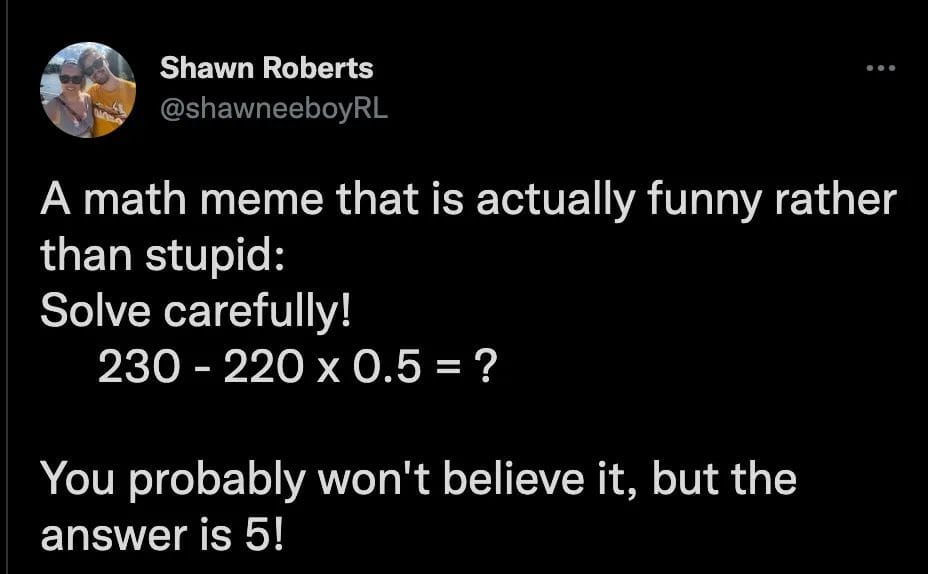
\includegraphics[width=0.7\linewidth]{pics/factorial}
	\caption{Hopefully you get it now.}
	\label{fig:factorial_meme}
\end{figure}



\subsection{Recursive Rules}

As previously mentioned, all recursive functions:
\begin{itemize}
	\item Must have one or more base cases where the solution is well defined.
	\item Must have one or more recursive cases, where the problem is defined by a smaller subproblem of the same type as the original.
	\item Must ensure the recursive cases make progress towards the defined base case.
\end{itemize}


You prove a recursive algorithm will solve the problem in question by showing all the above points are true.  
This is much the same as a proof by induction, just in the opposite direction.

\subsubsection{Failure to follow the rules.}

If your recursive case fails to make progress towards your base case, then you end up with a special type of infinite loop which is not actually infinite.  Every time you make a method call,  your computer needs to store where in the code it was and what conditions that were present.  The specifics of how and why this is done are outside the scope of the textbook \footnote{maybe}, but suffice to say, this information gets stored in a part of the computer memory designated as \textit{the stack}.  This stack is named such because it is a \texttt{Stack} just like what you have seen in Chapter \ref{chap-stacks}.  Since this stack is living in your memory and your computer probably does not have infinite memory  we can run the following program to see what happens when that stack ``fills up.''

\begin{javacode}{Recursion with no end condition - Java}
public static void bad(){
	bad();
}
\end{javacode}


\begin{pycode}{Recursion with no end condition - Python}
def bad():
	bad()
\end{pycode}

You'll get something along the line of a \texttt{Stack Overflow} error or exception, which indicates that your stack in memory has gotten completely used up.  This rarely happens in correctly created recursive programs.

\subsection{Fibonacci}

The Fibonacci sequence is the classic introduction to recursive formulas and recursion in programming.  I opted for teaching the factorial sequence first due to the complications with runtime a naive implementation has.  This might lead to the impression that \textit{all} recursive functions have a terrible runtime.  They do not.  





\subsubsection{History}
The Fibonnaci sequence is named after Leonardo Bonacci, also known as Leonardo of Pisa, and also known as Fibonacci.  He authored a book in 1202 called \textit{Liber Abaci}, which introduced the western world to calculations using Hindu-Arabic numerals .  It also enumerated the Fibonacci sequence, which is why it is named after him\cite{Bonacci1202,sigler2002fibonacci}.   Notice I said \textit{western} world.  It is hard to appreciate that humans could not share information in the same way we can today, as well as what can be lost due to damage or merely not writing it down.   The Fibonacci sequence had been observed previously by Indian mathematicians such as Gop\={a}la  \cite{singh1985fib}
Furthermore, it is completely possible someone had observed this sequence earlier, wrote it down in a text somewhere, and then the text being lost to fire or rot.  Backups are important and can mean the difference between having something named after you or not.

\subsubsection{Definition}
The Fibonacci sequence  (sequence A000045)\footnote{\href{https://oeis.org/}{Yes, humans are such nerds that we've created an online library for sequences - OEIS.}} is defined as the sequence of numbers where each number in the sequence is the sum of the previous two numbers.  The sequence starts with 0 and 1  and looks something like this:

$$0, 1, 1, 2, 3, 5, 8, 13, 21, 34, 55, 89, 144, 233, 377, 610, 987...$$

The sequence continues indefinitely. More formally, let $F_n$ be the $n$th number of the Fibonacci sequence. We define the sequence with:
$$ F_{0} = 1, F_{1} = 1$$
$$ F_n = F_{n-1} + F_{n-2}$$



Regardless, the Fibonacci sequence important.  It shows up again and again in nature, in science, and in mathematics.  The number of petals a flower has tends to be plucked from the Fibonacci sequence \cite{turner2020flowers}.
%TODO More Examples here


\begin{figure}
	\centering
	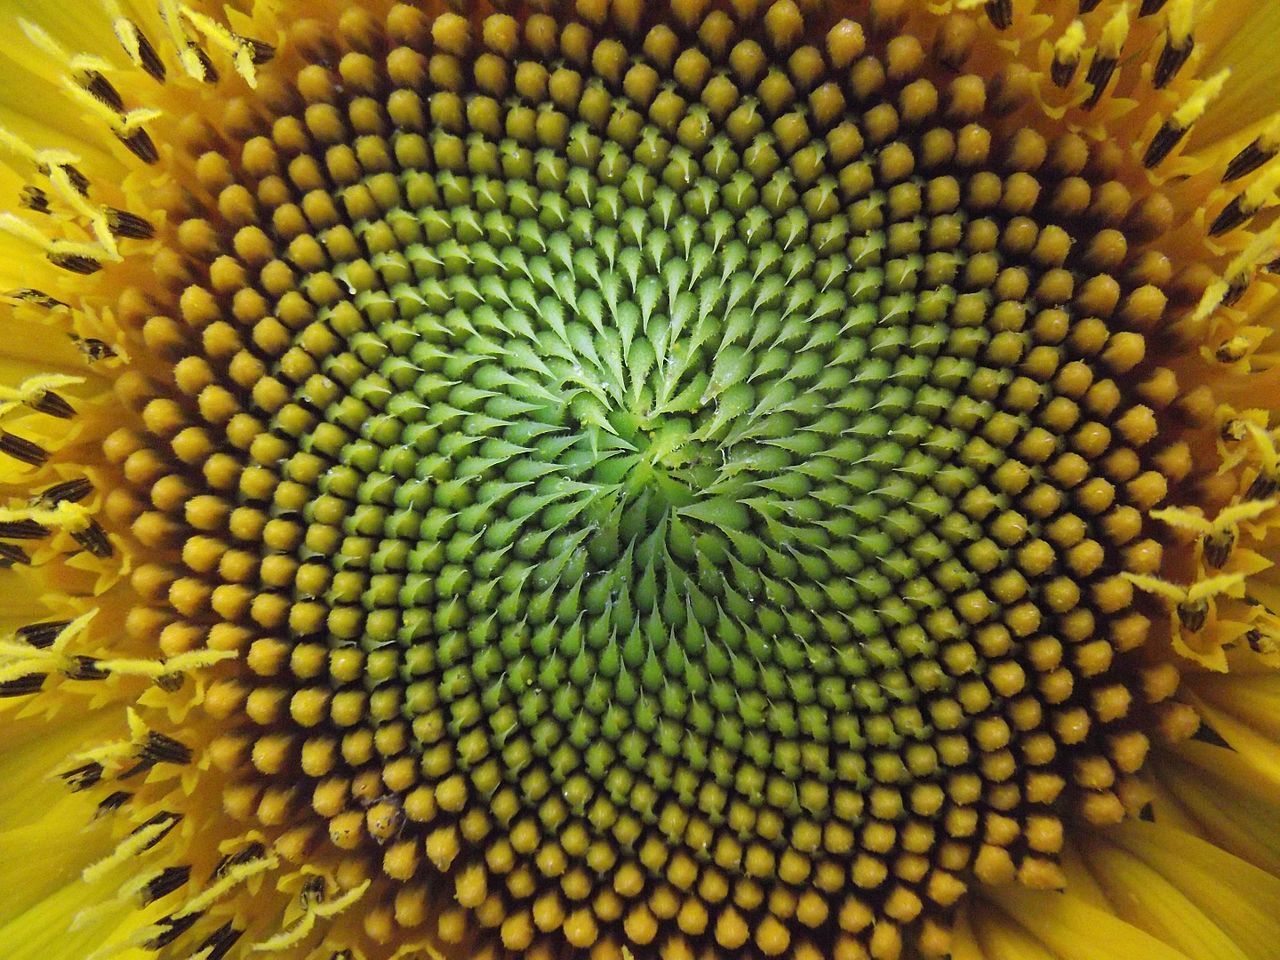
\includegraphics[width=0.7\linewidth]{pics/sunflower}
	\caption{The sunflower's fibonacci spiral. Photo by Anna Benczur, CC by-SA 4.0.}
	\label{fig:sunflower}
\end{figure}




\subsubsection{Implementation}
Implementing this as a recursive function is rather trivial!

\begin{javacode}{Naive Java Implementation}
public static long fib(int n){
	if(n == 0 || n == 1) {
		return n;
	}
	return fib(n - 1) + fib(n - 2);
}
\end{javacode}

\begin{pycode}{Naive Python implementation}
def fib(n):
	if n == 0 or n == 1:
		return n
	return fib(n - 1) + fib(n - 2)
\end{pycode}

\subsubsection{A Flaw appears in the plan}
As it turns out, while this technically works...it's pretty terrible.  In short, using recursion, I managed to accidentally\footnote{All right, I did this totally on purpose.} write an $ O(2^n) $, or exponential time, algorithm. This is very bad.  This means increasing $ n $ by one \emph{doubles} the runtime of out algorithm! Go ahead and try it for yourself on your computer.  You should start seeing some massive slowdowns when computing \texttt{fib(n)} somewhere around \texttt{n=45}.  Notice that each time you increase \texttt{n} by one, the amount of time your computer spends working roughly doubles.

This is because to solving the current \texttt{n} requires solving \texttt{fib(n-1)} and \texttt{fib(n-2)}.  Furthermore, each recursive call is independent from each other;  solving \texttt{fib(n-1)} 

\begin{figure}[h!]
	\centering
\begin{forest}
	for tree={
		grow=south, % Tree grows downwards
		s sep=5mm,  % Sibling separation
		l sep=10mm, % Level separation
		align=center, % Center align node text
		parent anchor=south,
		child anchor=north,
		font=\ttfamily, % Use a monospaced font for node text (already set, \texttt{} reinforces)
		edge={->}, % Arrow style for edges
	}
	[\texttt{fib(n)}
	[\texttt{fib(n-1)}
	[\texttt{fib(n-2)}
	[$\vdots$]
	[$\vdots$]
	]
	[\texttt{fib(n-3)}
	[$\vdots$]
	[$\vdots$]
	]
	]
	[\texttt{fib(n-2)}
	[\texttt{fib(n-3)}
	[$\vdots$]
	[$\vdots$]
	]
	[\texttt{fib(n-4)}
	[$\vdots$]
	[$\vdots$]
	]
	]
	]
\end{forest}

\caption{Recursive Function Calls for \texttt{fib(n)}.  Notice that the call to \texttt{fib(n-1)} must independently compute \texttt{fib(n-2)}, thus duplicating a ton of work.}
\label{fig:fibonacci_call_tree}

\end{figure}




\begin{figure}[h!]
\centering
\begin{forest}
	for tree={
		grow=south,
		s sep=5mm,
		l sep=10mm,
		align=center,
		parent anchor=south,
		child anchor=north,
		font=\ttfamily, % Use a monospaced font for node text (already set, \texttt{} reinforces)
		edge={->},
	}
	[\texttt{fib(4)}
	[\texttt{fib(3)}
	[\texttt{fib(2)}
	[\texttt{fib(1)}]
	[\texttt{fib(0)}]
	]
	[\texttt{fib(1)}]
	]
	[\texttt{fib(2)}
	[\texttt{fib(1)}]
	[\texttt{fib(0)}]
	]
	]
\end{forest}
\caption{Computing \texttt{fib(4)}.}
\end{figure}


Don't let this terrible runtime scare you away from recursion!  Recursion can make things quite efficient; this is merely an exception and presented here because Fibonacci is such a classic example we would be remiss to not include it.  

\subsubsection{Solutions}
There's a lot of solutions to make this work.  My personal favorite is \textbf{memoization}, which simply says ``well if the issue is having to redo the work, let's instead store the results of each function call.''



\begin{javacode}[listing and comment, comment={So here we have a public method that the programmer will use to calculate the \texttt{n}th Fibonacci number and a private helper method to do the actual work.  The array \texttt{F} is an array where we store any previously calculated Fibonacci numbers.  The big change from our original solution is now we ask if the \texttt{n-1} Fibonacci number has been calculated before.  If it has not, calculate it and store it in the array.  We do the same for the \texttt{n-2} Fibonacci number. The reference to the array is shared  between all recursive calls.  After the check and the possible calculation is done, the function uses those numbers to calculate \texttt{fib(n)}.}] {An Efficient Recursive Fibonacci Algorithm}
public static long fib(int n) {
	long[] lookup = new long[n];
	lookup[1] = 1;
	return fib(n , lookup);
}


private static long fib(int n, long[] F) {
	if(n <= 1) { //base case
		return F[n];
	}
	if(F[n-1] == 0) {
		F[n-1] = fib(n-1, F);
	}
	if(F[n-2] == 0) {
		F[n-2] = fib(n-2, F);
	}
	return F[n-1] + F[n-2];
}
\end{javacode}


\begin{pycode}[listing and comment, comment={So here we have a function with a default variable \texttt{F} that is initially an empty list.  If the program detects \texttt{F}'s empty, it is initialized to a list of zeroes.  We do this to avoid writing a second function, like we did in the Java example. The list \texttt{F} is a list where we store any previously calculated Fibonacci numbers.  The big change from our original solution is now we ask if the \texttt{n-1} Fibonacci number has been calculated before.  If it has not, calculate it and store it in \texttt{F}.  We do the same for the \texttt{n-2} Fibonacci number. The reference to \texttt{F} is shared  between all recursive calls.  After the check and the possible calculation is done, the function uses those numbers to calculate \texttt{fib(n)}.}]{An Efficient Recursive Fibonacci Algorithm in Python}
def fib(n, F = []):
	if len(F) == 0:
		F = [0] * n
	if(n <= 1):
		return n
	if(F[n - 1] == 0):
		F[n - 1] = fib(n - 1,F)
	if(F[n - 2] == 0):
		F[n - 2] = fib(n - 2,F)
	return F[n - 1] + F[n - 2]
\end{pycode}



\section{More Examples}
Some of the upcoming examples  of the things we are about to see should not be actually  used and serve only as examples, like our \texttt{printThis} function.

\subsection{Printing Recursively}

\begin{javacode}{Recursive Printing: Java}
public static void printThis(String s){
	if (s.length() == 0) {
		System.out.println();
	} else {
		System.out.print(s.charAt(0));
		printThis(s.substring(1));
	}
}
\end{javacode}

\begin{pycode}{Recursive Printing: Python}
def printThis(s):
	if len(s) == 0:
		print()
	else:
		print(s[0], end='')
		printThis(s[1:])
\end{pycode}


\section{Arrays with Recursion}


\subsection{Summation of an Array}
%%https://runestone.academy/ns/books/published/javads/recursion_calculating-the-sum-of-a-list-of-numbers.html
%ADD REFERENCE HERE
%
%
%We will begin our investigation with a problem that you already know how to solve without using recursion. Suppose that you want to calculate the sum of an array of numbers such as:$[1, 3, 5, 7, 9]$ An iterative method that computes the sum is shown in Listing 4.3.1. The method uses an accumulator variable (theSum) to compute a running total of all the numbers in the array by starting with and adding each number in the array.


The ay to think of this is in terms of a base case and a recursive case.  The base case is size of one or zero.  Either way, the answer is trivially easy to figure out.  The recursive case is basically a way of saying adding a bunch of numbers is too hard.  I'll just return adding the number at the first index of this section or subsection of the array to whatever the total the rest of the array is.  I'll use a magic function to figure it out.  it turns out the magic function is actually this one.


\subsection{Recursive Linear Search}

By this point, you know how to iteratively search a list for a specific item.  We start at the first item/index and go thru the array one item at a time until we get to the last item or find the item we want.   Let's take a look at the same algorithm, just implemented recursively.


\begin{javacode}{Recursive Linear Search - Java}
// We return the index we found the item at
// -1 means item is not in the list
public static <E> int search(List<E> list, E target){
	return search(list, target, 0);
}

private static <E> int search(List<E> list, E target, int index) {
	if(index >= list.size()){
		return -1;
	}
	if(list.get(index).equals(target)){
		return index;
	}
	return search(list,target, index+1);
}
\end{javacode}

\begin{pycode}{Recursive Linear Search - Python}
def search(theList, target):
	return search(theList, target, 0)

def search(theList, target, index):
	if index >= len(theList):
		return False 
	if theList[item] == target:
		return True
	return search(theList, target, index + 1)
\end{pycode}



Again, this is more of a case of pedagogical examples, rather than practical ones.  We want to get some practice in before we get to the really interesting recursive problems.  

\subsubsection{Runtime}  
The above code has the exact same runtime as doing it iteratively -- $O(n)$ in the case of an \texttt{ArrayList}. Remember, we don't want to use this for a \texttt{LinkedList} due to the $O(n)$ cost the \texttt{get} method incurs, which would yield an overall $O(n^2)$ runtime. Use the built-in iterator instead, i.e. use a for each loop.
\subsection{Binary Search}
Binary search is our reason for including Recursion at this location in the textbook.   It will be an essential step in building Binary Search Trees.


\subsubsection{Objective}
Like our recursive linear search, our goal is to search for a particular item in an array or list.  Once we find that item, we can either return true or the index we found it at, depending on our implementation.  If we fail to find, we return either false or -1 or \texttt{null}; again this depends on our implementation.\footnote{ \href{https://scryfall.com/card/chk/62/gifts-ungiven}{Or force a win using \textit{Gifts Ungiven}}.  Wait, wrong fail to find.}.

\subsubsection{Assumptions}
We will be using an array for Java and \texttt{List} for Python.  This data structure will be sorted.  This is a key assumption;  if the array is not sorted, we cannot do a binary search.

\subsubsection{Solution}
Since our core assumption is that we are using a sorted collection, it makes sense that our algorithm exploits this.  Think of a game that you might have played in school as a kid, the ``I'm thinking Of a number from one to 100. I'll tell you if it's higher or lower.''  Now the linear strategy that we went over previously would be the equivalent of asking ``Is it one? Oh, it's higher? Is it 2? It's higher? Is it 3? Oh, it's higher?'' and so on and so forth Until we hit the number in question. A more reasonable strategy would be to pick the number 50 because that number is in the middle of the entire range.  Once we know whether the number is higher or lower we have effectively halved our range. This is because if the number is higher than 50 we know that the number cannot be between 1 and 50, inclusive. If it is lower than 50 we know the number cannot be between 50 and 100, inclusive.   And if the number is 50 we just simply got lucky.
The next step is to choose the number in the middle of our new range so we can do the same halving of our search space.

Let's take this strategy and apply it to an array of sorted numbers, seen in Figure \ref{fig:binarysearch1}.

 
\begin{figure}[h!]
	\centering
	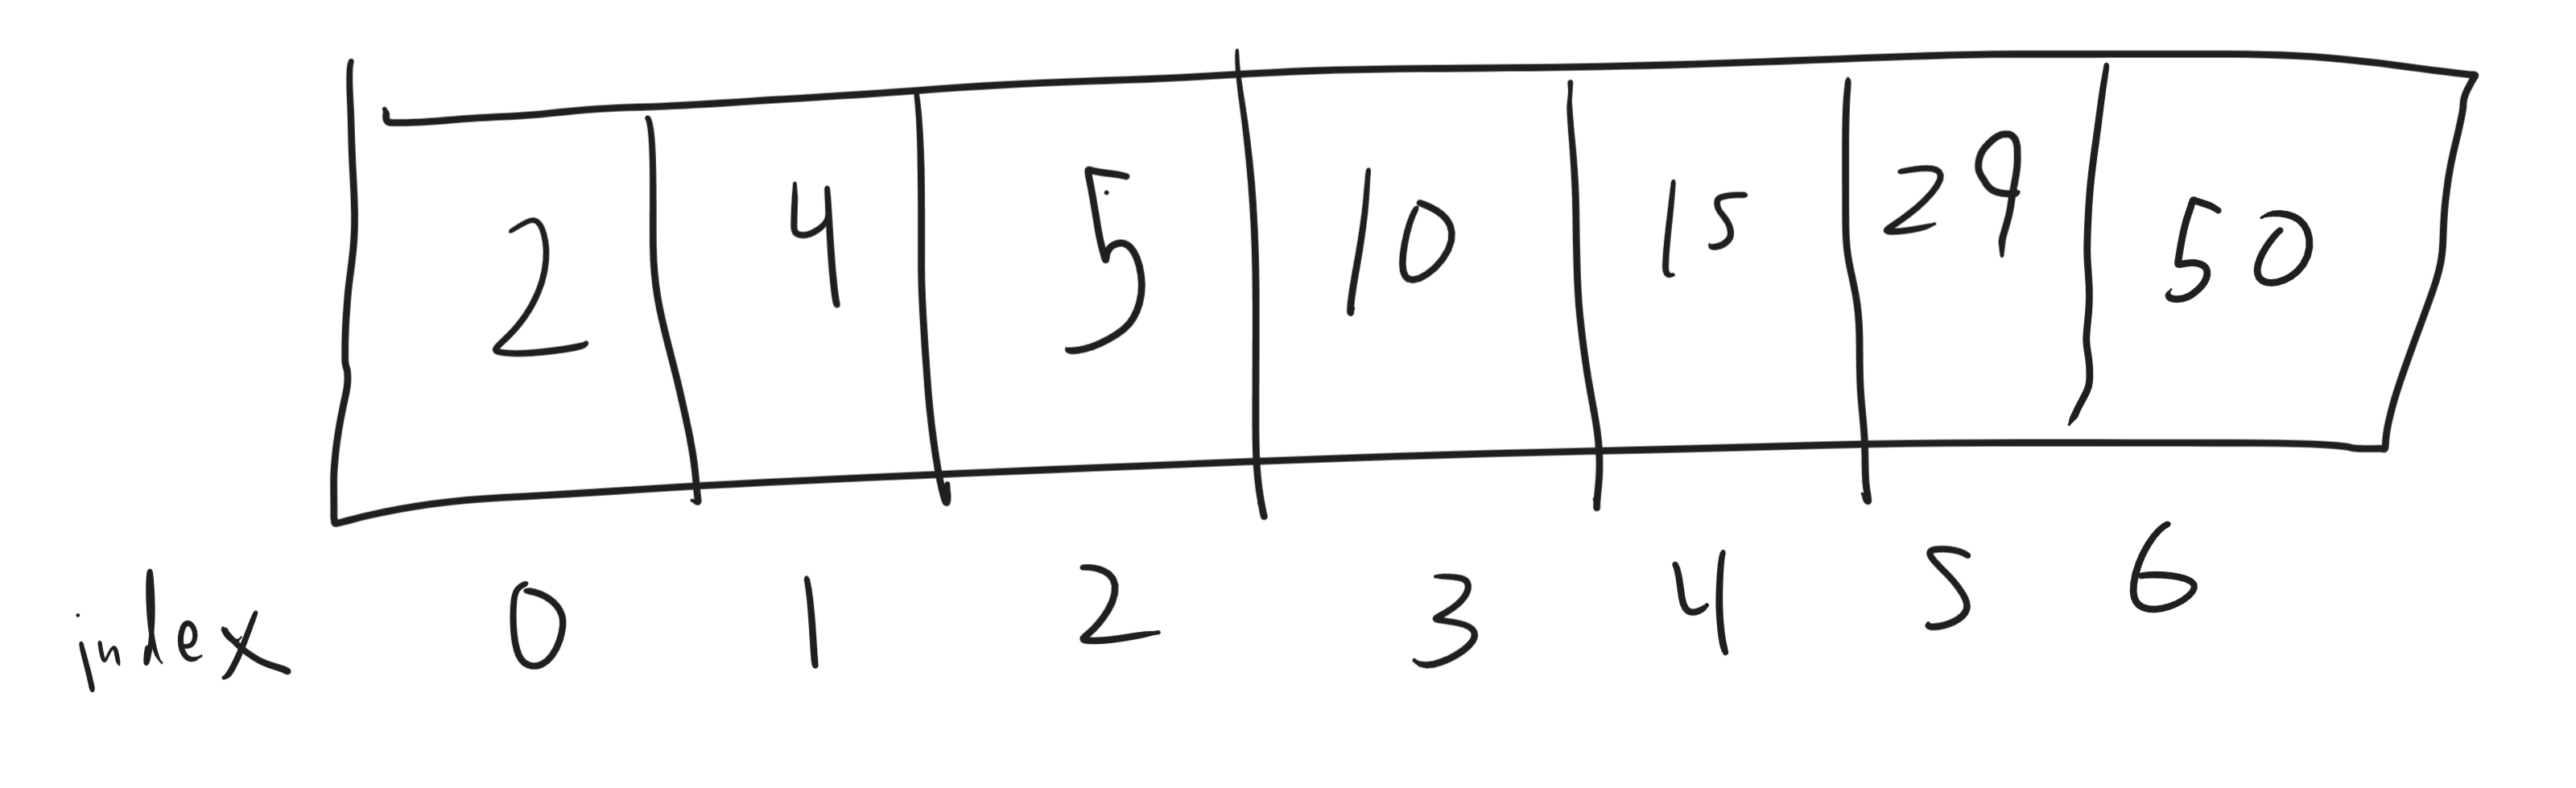
\includegraphics[width=0.7\linewidth]{pics/binarySearch1}
	\caption{}
	\label{fig:binarysearch1}
\end{figure}


In this example, we want to see query if this array contains the item $5.$   We start by asking figuring out what the middle index of the array is, since half the items in the array will be to the left and half to the right\footnote{Or half stored in lower indices and half stored in higher indices if you prefer.}.  The array is 7 items total, so we start at index 3  and compare 5 to the value stored in there (Figure \ref{fig:binarysearch2}).

\begin{figure}[h!]
	\centering
	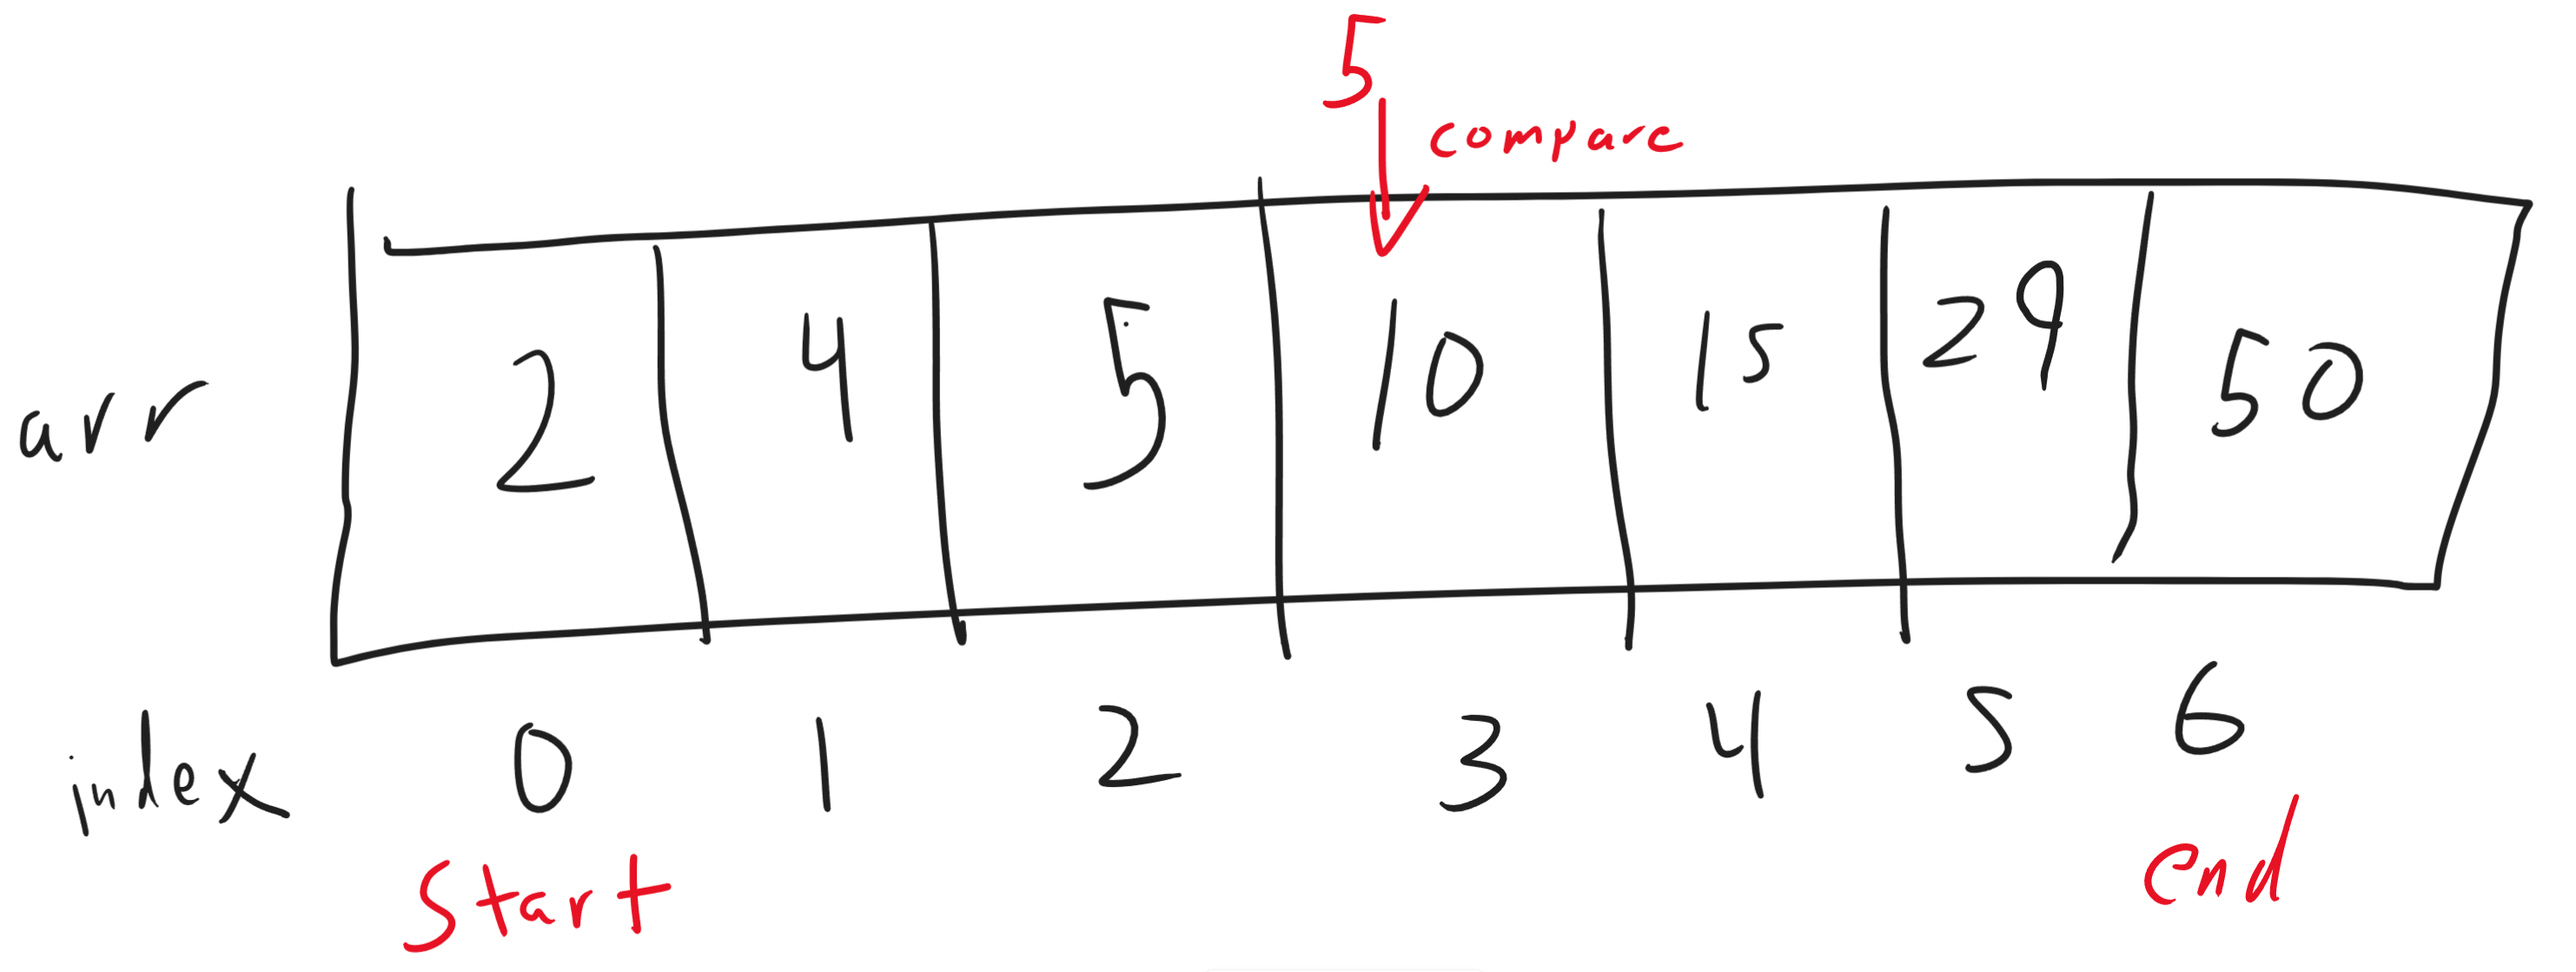
\includegraphics[width=0.7\linewidth]{pics/binarySearch2}
	\caption{The labels \texttt{start} and \texttt{end} represent the start and end of our search space.  This will make more sense as we progress, especially as we start coding.}
	\label{fig:binarysearch2}
\end{figure}

Since $5 < 10$, we know that if 5 is in the array, it will be found to the left of index 3.  We put the end of our search space one index to the left of the middle of our previous search space.  Our new range to search is now index 0 thru index 2 (Figure \ref{fig:binarysearch3}).  We compare 5 to the item in the middle of that range, which is the number 4 at index 1.  



\begin{figure}[h!]
	\centering
	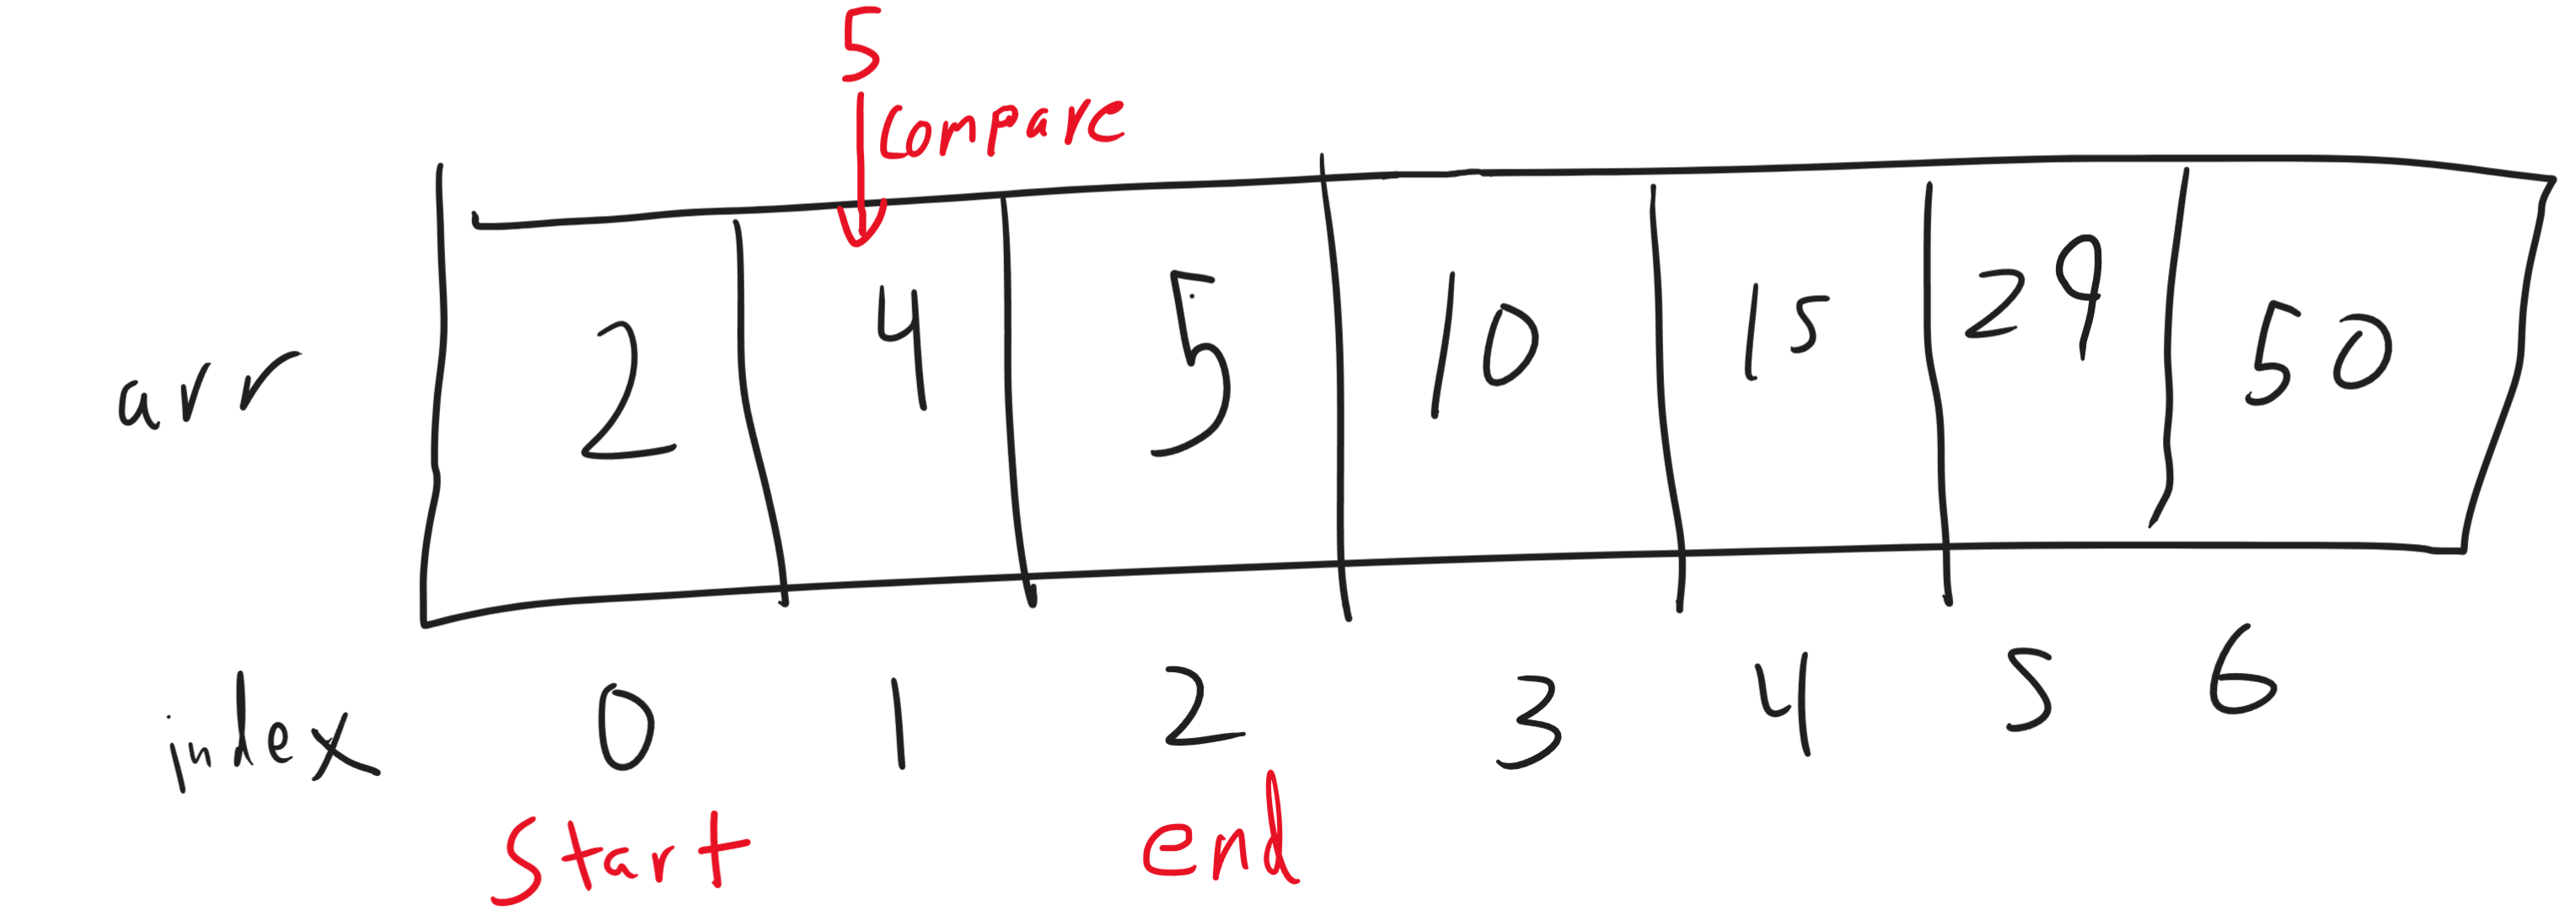
\includegraphics[width=0.7\linewidth]{pics/binarySearch3}
	\caption{The labels \texttt{start} and \texttt{end} represent the start and end of our search space, which has now shrunk to less than half the original array.}
	\label{fig:binarysearch3}
\end{figure}

$5 > 4$, so if 5 is in the array, it is on the right side of our search space.  Our search space contracts to a single item, index 2 (Figure \ref{fig:binarysearch4}).  

\begin{figure}[h!]
	\centering
	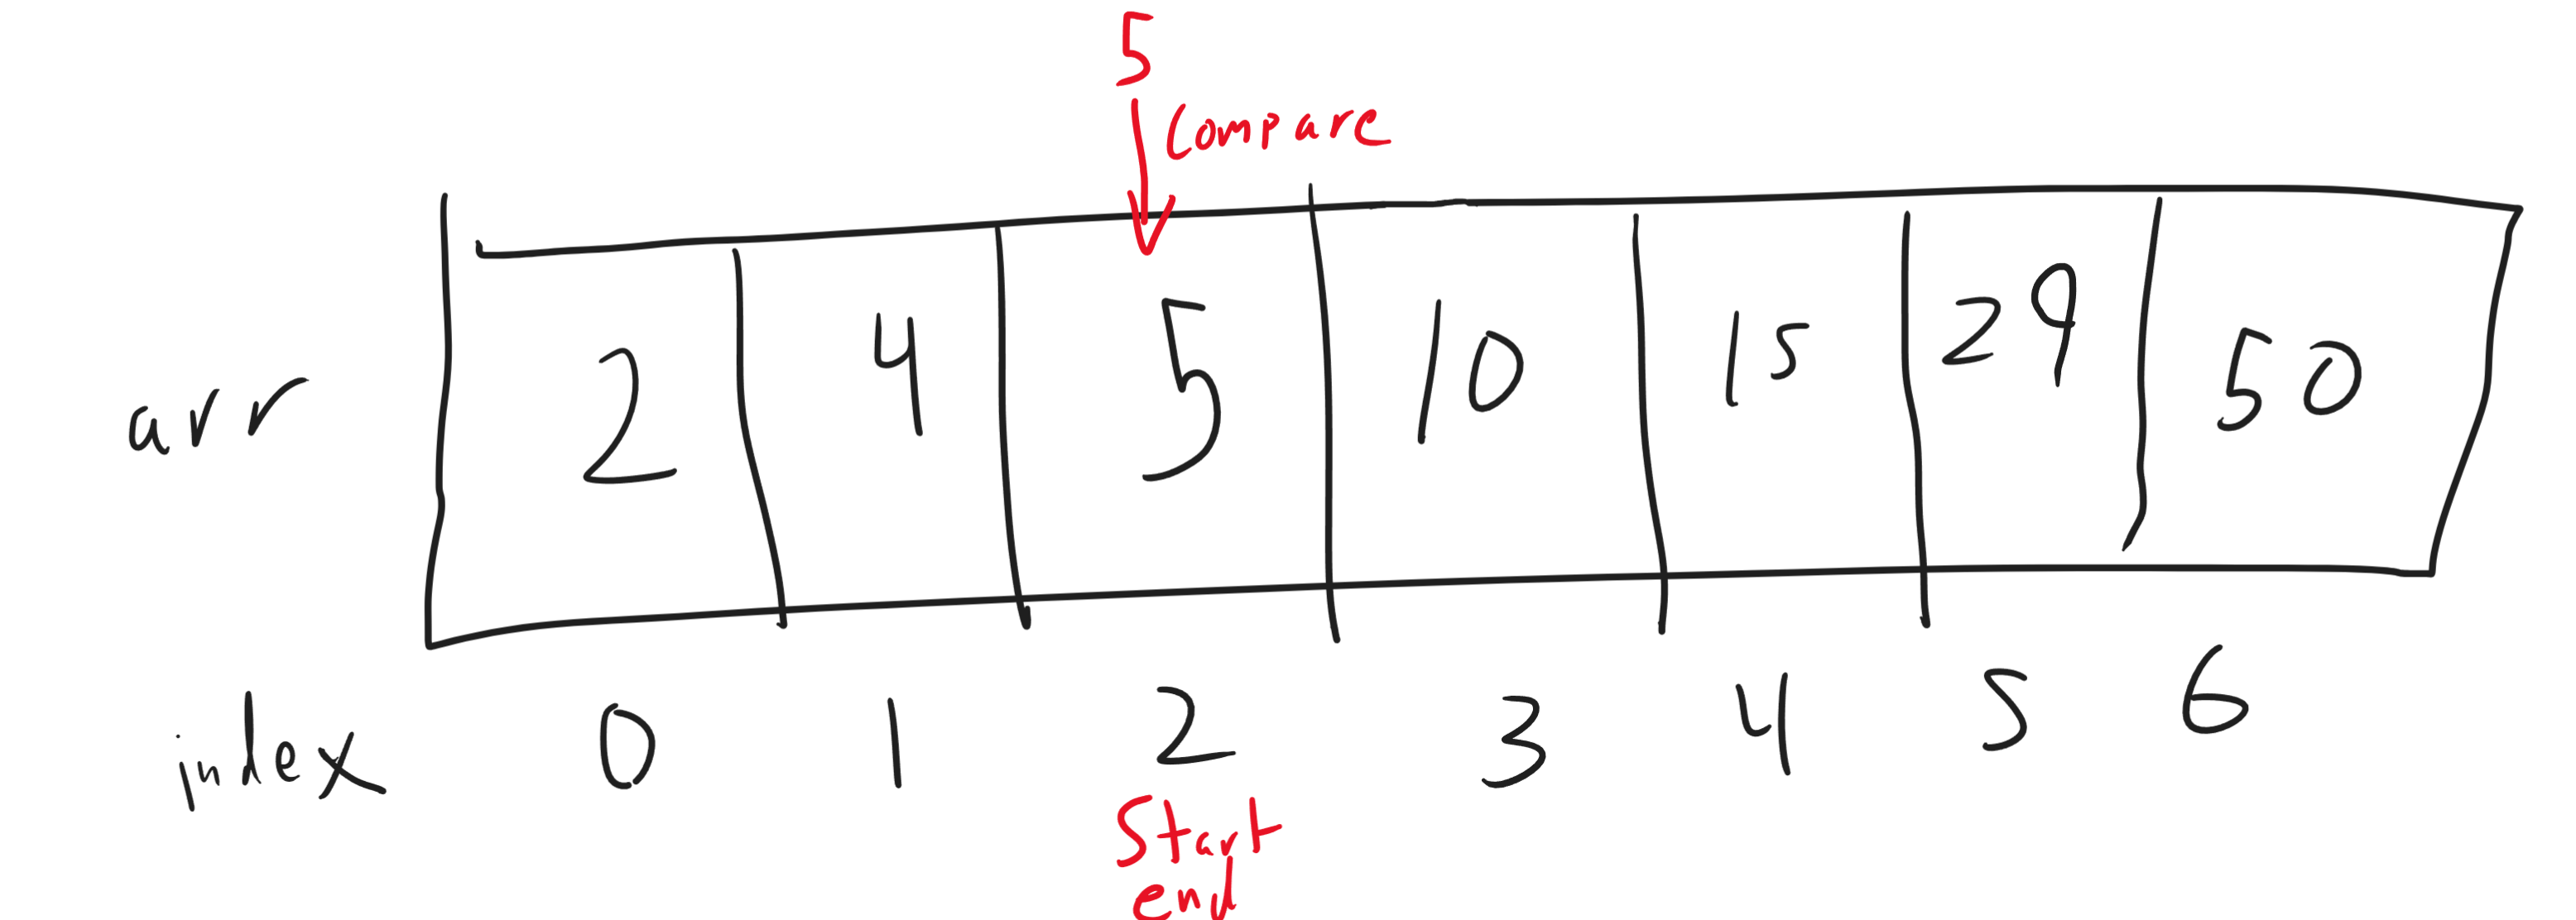
\includegraphics[width=0.7\linewidth]{pics/binarySearch4}
	\caption{The labels \texttt{start} and \texttt{end} are now on the same item.  This means a search space has a size of 1.}
	\label{fig:binarysearch4}
\end{figure}


The item at index 2 is the same item we've been looking for, so we have successfully found our item.

\subsubsection{Code}



\begin{javacode}[listing and comment, comment={Our outer, wrapper function exists to have a clean function to call.  Our helper function does the actual work.  If we fail to find our target, we will return -1, which is an invalid index.}]{Binary Search - Java}
public static int binarySearch(int[] arr, int target) {
	return binarySearch(arr, target, 0, arr.length-1);
}

private static int binarySearch(int[] arr, int target, int start, int end) {
	if(start > end) {
		return -1;
	}
	int mid = (start + end) / 2;
	if(target == arr[mid] ) {
		return mid; // item found
	} else if( target < arr[mid]) {
		// search right side
		return binarySearch(arr, target, mid+1, end);
	} else {
		// search left side
		return binarySearch(arr, target, start, mid-1);
	}
}
\end{javacode}


\begin{pycode}[listing and comment, comment={Here, we have two base arguments for our initial call, with start and end to be used for a recursive call.  The first if statement is to set \texttt{end} correctly for our topmost (initial) call, because I'm too lazy to write a second, private helper function.  The first base case returns \texttt{None} to represent a failure to find.}]{Binary Search in Python}
def binarySearch(arr, target, start = 0, end = 0):
	if len(arr) > 0 and end == 0:
		end = len(arr) - 1
	if start > end:
		return None
	mid = (start + end) // 2
	if arr[mid] == target:
		return mid
	elif target < arr[mid]:
		return binarySearch(arr, target, start, mid - 1)
	else:
		return binarySearch(arr, target, mid + 1, end)
\end{pycode}

In our above code, we create two base cases, which are quite simple if you think about it.  The first is if our search space is size 0 or invalid.  We obviously can't find \texttt{target} in the search space if the search spaces doesn't exist. This is the \mintinline{Java}|if(start > end)| clause, since if the start of the search space is to the right of the end of the search space, we don't have a valid space to search anymore.  In this scenario, we return a failure state of some sort\footnote{-1 in our Java example and \texttt{None} in our python example.}.  

The next step is to calculate \texttt{mid} which is the index in the middle of the search space.  From there, we get our second base case:  if the item at index \texttt{mid} is the item we are looking for, we're done.   Otherwise, we check if \texttt{target < arr[mid]}.  If this is true, then target must be on the left half of the array.  To search that left half for \texttt{target}, we call \texttt{binarySearch(arr, target, start, mid - 1)}.    Why are each of the arguments what they are?

\begin{itemize}
	\item The first parameter of \texttt{binarySearch} is the array or list we are search, so the argument that we pass into our recursive call remains the same.
	\item The second parameter is the \texttt{target} item, which remains constant.
	\item The third parameter is the beginning index of our search space.  When we search to the left side of the search space, we are searching between \texttt{start} and \texttt{mid}, not including \texttt{mid}.  Thus the third argument won't change.
	\item We pass in \texttt{mid - 1} as the \texttt{end} of the new search space, since that is the right side of the new, smaller search.
\end{itemize}


Now, if  \texttt{target < arr[mid]} is false, we search the right side, which means that the fourth argument is \texttt{end}, but we change the third argument to \texttt{mid + 1}.


%TODO Lazy Thinking comparison


\subsubsection{Runtime Analysis}
Each call of \texttt{binarySearch} eliminates either exactly or almost exactly half of the search space if we don't find our \texttt{target}.  This halving can be mathematically  described by the operation $\log_2(n)$, where $n$ is the number of items.\footnote{If the sudden appearance of logarithms risks scaring you off, just keep reading to the next subsubsection.  I wrote that special for you.}  Thus, with an array of 256 items, this algorithm would take approximately 8 steps. Doubling the size of the array to 512 items increases the amount of work only by a single step. This yields $O(\log n)$  as the runtime.\footnote{ We drop the base of a logarithm when we use big $O$ notation.}    
 
Compare that to our linear search, which starts at the beginning and goes through the array one item at a time. That takes $O(n)$ time. In this case, doubling the number of items means doubling the amount of work the algorithm has to do.

It bears emphasizing and repeating:  $O(\log n)$ runtime is a major improvement over a linear runtime.  Doubling the size of $n$ does practically nothing to change the runtime of \texttt{binarySearch}, but would make a linear search take twice as long.


\subsubsection{How to not be scared of logarithms}
You may have learned that logarithms are the inverse operation to exponentiation.
This is an utterly useless definition when programming.

A much more useful way of thinking about logarithms is ``how many times can I recursively split something?''
For example, $\log_b x$ asks ``how many times can I recursively split my $x$ items into $b$ seperate piles?''

A more concrete example: $\log_2 16 = 4$, not because $2^4 = 16$, but because a pile of 16 items can be split in half into two piles of 8, each pile of 8 can be split in half into two piles of 4, the 4's can be split into 2's, the 2's into 1's --- four splits total:

\begin{figure}[h!]
	\centering
	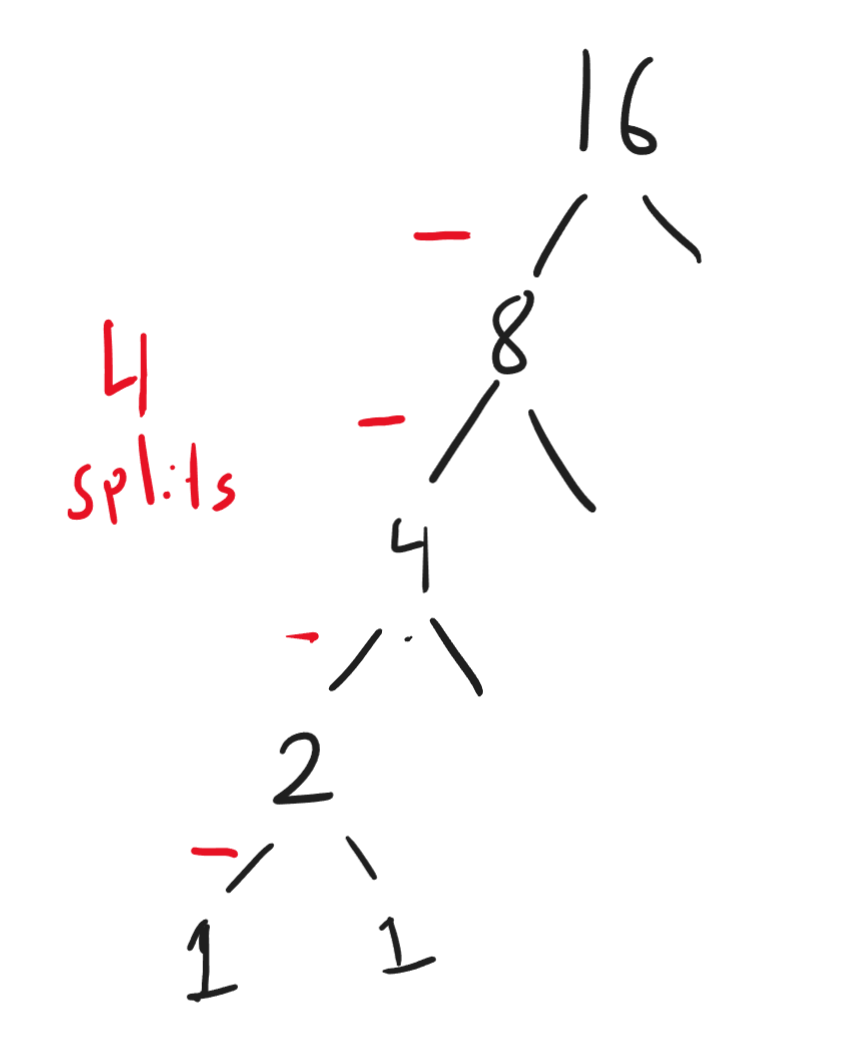
\includegraphics[width=0.4\linewidth]{pics/log16}
	\caption{}
	\label{fig:log16}
\end{figure}



In algorithm analysis, $\log n$ in the time complexity is used to indicate that the search space gets split in half.
In the Binary Search algorithm above, we split the our search space in half each step of the way.  We start out looking at the middle item and then decide to look at all the items below or all the items above.  This reduces the number of items to search among from $n$ to $\frac{n}{2}$.  From there we perform the same choices and reduce that $\frac{n}{2}$ to $\frac{n}{4}$, then from  $\frac{n}{4}$ to  $\frac{n}{8}$ and so on.

\subsubsection{Additional Implementation: Java with Lists}
\label{sec:binarySearchJavaP2}


\begin{javacode}[listing and comment,  comment={Performing binary search on a list looks something like this.  Recall that \texttt{Comparable} is an interface that Java uses to let methods and classes know something can be put in order\footnote{Formally, this is a  \textit{total ordering} in fancy math lingo, which means any two items have an established order}.  This necessarily  means that they can be sorted. The generic \texttt{<E extends Comparable<E>>} means the the \texttt{List} of \texttt{E}'s is guaranteed to be made up of items that can be compared to other things of type \texttt{E} to see which comes first.}]{Binary Search - Java Lists}
public static <E extends Comparable<E>> int binarySearch(List<E> list, E target) {
	return binarySearch(list, target, 0, list.size()-1);
}

public static <E extends Comparable<E>> int binarySearch(List<E> list, E target, int start, int end) {
	if(start > end) {
		return -1;
	}
	int mid = (start + end) / 2;
	if(target.compareTo(list.get(mid)) == 0) {
		return mid; // item found
	}
	if(target.compareTo(list.get(mid)) < 0) {
		// search right side
		return binarySearch(list, target, mid+1, end);
	} else {
		// search left side
		return binarySearch(list, target, start, mid-1);
	}
}

\end{javacode}

\section{Recursive Backtracking}
Recursion really comes in handy when we are trying to solve complex puzzles.
One of the most famous examples of this is using recursion to solve the eight queens problem or Sudoku.  Before we get into this, let's establish the rest of the chapter. I'll introduce the eight queen's puzzle.  Then, I'll show you the generic recursive backtracking algorithm, explain it, and then show a partial solution to the eight queens puzzle.  I'll also go over the Sudoku solver, but will leave that as a potential homework.


The entire reason for this aside is to speak to both the students and instructors who use this book.  The eight queens problem is a recursive problem that has been used as a homework problem longer than I've been alive.  This means there are a million and a half solutions floating around the internet.  

Students: I ask you do not rob yourself of that learning experience and instead strive to follow the text I have here.   Go to your teacher or TA or classmate if you get stuck for more than two hours.  

Teachers:  Give these exercises, or something similar like the knight's tour, as a homework assignment.  These are engaging and worth it.  Yes, some students are going to completely ignore the plea of the last paragraph, but they were going to do that no matter what assignment you gave.  Don't rob the engaged students of a great learning experience.

\subsection{The Eight Queens Puzzle}
The eight queens puzzle is an old chess puzzle. If you don't know how to play chess, you should change that, but knowing how to play is not necessary to solving the puzzle.  

The goal of the puzzle is to place eight queens on a standard $8 \times 8$ chessboard.  The queens should be placed in such a way that no queen can capture any other queen.  In chess, a queen can capture any piece by traveling vertically, horizontally, or diagonally until it crashes into a piece.  Or in more programming friendly terms, we need to place 8 queens such that none share a row, column, or diagonal.

This is one example solution, but it is not the only solution.



\chessboard[setwhite={Qa1,Qb7,Qc4,Qd6,Qe8,Qf2,Qg5,Qh3},showmover=false]

\subsubsection{Brute Force Solution}
A brute force algorithm means we will be checking every single possible state to find a solution.
In this case, a brute force solution for the Eight Queens Puzzle would every possible placement of eight queens on a chessboard, such as  these two incorrect solutions:

\chessboard[setwhite={Qa2,Qb7,Qc2,Qd6,Qe8,Qf4,Qg5,Qh3},showmover=false]

\chessboard[setwhite={Qa2,Qb7,Qc2,Qd6,Qe8,Qf2,Qg5,Qh3},showmover=false]

There are a total of $\binom{64}{8} = 4426165368$
possible ways to place 8 queens on a chessboard with 64 spaces.  Our computer could sift thru all possible configurations until it finds a solution, and thus, performing a brute force solution will eventually work. It just won't work fast.

Our motive is to do better and apply some more logic to our searches.
Take those two incorrect solutions, for example.  The first has queens on spaces a2 and c2, which means that it is an incorrect solution.  The second example also has queens on a2 and c2, but additionally it has a queen on f2.  
If we can go about finding a solution more methodically, there is no reason that we should ever check the second example.  
Once we establish that placing a queen on a2 and c2 doesn't work for a solution, we should never check any solution that contains a2 and c2 ever again.
If fact, let's try and go even further. Assume to generate a solution,we place queens right to left, going one column at a time, like so:

\chessboard[setwhite={Qa2},showmover=false]

\chessboard[setwhite={Qa2,Qb7},showmover=false]


\chessboard[setwhite={Qa2,Qb7,Qc2},showmover=false]

Once we hit this point, there is no need to place any more queens, since we know any of the remaining 5 queens we place down will be in a ``dead'' branch of the search space.  This would allow us to ``skip'' checking the $\binom{40}{5} = 658008$ solutions that place the five other queens.
\subsection*{The Recursive Backtracking Algorithm}
So how do kill a branch of our search space off?  

We're going to generalize the puzzle for our next step.  Let's introduce you to \texttt{solve}, our recursive backtracking algorithm.

\begin{minted}[style=bw]{C}
boolean solve(board,  pos){
\end{minted}


This solve method will take in two parameters: \texttt{board} and \texttt{pos}.  Board is the puzzle we are trying to solve and all the work we've done on it so far.  In eight queens, it will be our chess board and where we've paced the queens.  For Sudoku, it would be the grid and all the numbers we have put down (more on that later).  For a maze, such as in Chapter \ref{sec:mazes}, this would be the configuration of the maze, e.g. the walls and corridors and any marks we have made to avoid searching the same thing twice. 

Now, \texttt{pos} is our \textit{position} in the puzzle. Let's think of it as the current thing we are trying to solve.  For the Eight Queens puzzle, our position the current column we're placing our queen on (more on that later).  For Sudoku, we need to find what number goes in this current square. In the maze, we want to select the path leads to the end.


Finally, the \texttt{boolean} return value is used to signal whether solved the puzzle or failed.

So now that we are given the two parameters we need, we need to come up with a nice, concise algorithm that solves the entire puzzle.  That's a bit of a tall order, but since we are in the Recursion chapter, we should probably think of a recursive solution\footnote{  \href{https://en.wikipedia.org/wiki/Metagame}{Metagaming} is a valuable skill in not just in games, but in school and life.  Don't just study the material is for the exam, predict kind of questions your Professor likes to asked based on prior knowledge.}.   That's good, because that will enable us to be \textit{lazy}.


Our recursive solution requires the two elements all recursive solutions need -  a base case and a recursive case.  We'll also find we need a third case, but more on that in a bit.


\begin{minted}[style=bw]{C}
boolean solve(board,  pos){
	// base case
	
	// recusive case
}
\end{minted}

Let's start with the base case.  The base case should be the simplest, laziest thing we can think of.  For any puzzle, that would be the board already being solved.  If our position indicates everything is done, we return true to signal that the maze is solve.  This would be having no queens left to place, or no Sudoku squares to fill, or having found the exit.

\begin{minted}[style=bw]{C}
boolean solve(board,  pos){
	// base case
	if(pos indicates puzzle is solved){
		return
	}
	// recusive case
}
\end{minted}

Easy.  Now onto the recursive case.  The puzzle is not solved.   So let's do the \textit{next laziest} thing  - solving our current position, the bare minimum.  Now at our position, we have lots of possible choices.    


We can think of it as which choice is needed to make to solve the \textit{entire} puzzle from here.  Where do we need to put the queen so it will be valid for all the other choices?  What number is the correct number to put in this square?  What turn in the maze will lead us to the exit?  There is no way to know if we're not at the base case, but we're going to pretend that the choice we're making is the correct one for now.

What makes this better than brute forcing a solution is that not every possible choice we can make is valid. How do we figure that out which choice is valid?  That depends on the puzzle, so we are going to be lazy and abstract checking if a choice is valid to a \texttt{valid} function.

This brings us to the first part of the recursive step. Look at each choice we can make, one at a time.  As soon as we find a valid choice, we're going to pick it and assume it's correct.

\begin{minted}[style=bw]{C}
boolean solve(board,  pos){
	// base case
	if(pos indicates puzzle is solved){
		return
	}
	// recusive case
	for each possible choice {
		if(valid(choice)){
			select and mark that choice;
			// part two goes here
		}
	}
}
\end{minted}


This next part is the trickiest when we first look at it, but once we get the hang of it, writing \texttt{valid} will be the hardest part of doing this kind of algorithm.

Now that we've made our presumably correct choice, we are going to be lazy and call a magic \texttt{solve} function to solve the rest of the puzzle from the next position.  That function will return true or false, depending on whether the magic \texttt{solve} function found a solution or not.  If it returns true, we will return true to indicate to whatever function called us that the puzzle is solved with the found solution stored in \textit{board}.

If \texttt{solve} returns false, that's going to indicate this choice will not lead to a solution, given the current state of the \textit{board}.  When that happens, we will need to undo whatever we did to mark our current choice and resume checking the other possible choices to find if one is valid.


\begin{minted}[style=bw]{C}
boolean solve(board, pos) {
	// base case
	if(pos indicates puzzle is solved) {
		return
	}
	// recusive case
	for each possible choice {
		if(valid(choice)) {
			select and mark that choice;
			if(solve(board, nextPos) == true){  // recursive case
				return true;
			}
			unmark board at pos if needed, as choice was invalid;
		}
	}
	// But what if there's no valid choice?
}
\end{minted}


As it happens, the magic function to solve the rest of the puzzle is the one we are currently writing, so we're almost done.

Unlike our previous recursive problems which only had a base case and a recursive case,  our solution involves a failure state of sorts.   What if we look at all our choices and none of them work? If we hit this case, our program knows it won't be able to find a solution with the current configuration and uses \mintinline{Java}|return false| to inform the function that called it that something in the current configuration needs to change.


This failure case is what makes this a recursive backtracking algorithm.


\begin{minted}[style=bw]{C}
boolean solve(board, pos) {
	// base case
	if(pos indicates puzzle is solved) {
		return
	}
	// recusive case
	for each possible choice {
		if(valid(choice)) {
			select and mark that choice;
			if(solve(board, nextPos) == true){  // recursive case
				return true;
			}
			unmark board at pos if needed, as choice was invalid;
		}
	}
	return false; // backtrack
}
\end{minted}
	
As I previously mentioned, while this looks complicated at first, especially the \texttt{if(solve(board, nextPos) == true)}  once we get used to it, the recursive part is fairly straightforward.


A\textbf{ key feature }of this is that we always know where we are;  we never have to search for the space we are trying to solve - it is the current position.


\subsection{Recursively Solving the Eight Queens Problem}

Now that we have generalized algorithm, let's apply it to the Eight Queens problem.  
We'll represent the chess board as a 2D array.  There's many different valid type we could use, but I'm going to use an array of \texttt{String}, using \texttt{'Q'} and \texttt{'-'} to represent a space with a queen and an empty space respectively.  Our position in the puzzle with be the \texttt{col} variable, representing the column we are currently working on.  Finally, the choice for each column will be what \texttt{row} we place the queen on.

\begin{javacode}[listing and comment, comment={The initial call to solve will pass in \texttt{0} for \texttt{col} to start at the first column. We use \texttt{col == 8} as the base case, as a call to \texttt{solve(board, 8)} would be trying to check a column that does not exist.  The only way for that to happen is from a call on the  8th column (index 7), which means that that last column has found a working solution. If we want to generalize this solution to work on square boards other that a standard 8x8 chess board, we can do that by replacing all the 8's in the code with \texttt{board.length}.}]{Outline of Solution - Java}
public static boolean solve(String[][] board, int col){
	if(col == 8) { // use board.length to generalize
		return true;
	}
	
	for(int row = 0; row < 8; row++) {
		if(valid(choice)){
			place "Q" at row,col
			if(solve(board, pos + 1) == true){
				return true;
			}
			replace "Q" with "-", as choice was invalid
		}
	}
	return false; // backtrack
}
\end{javacode}


\begin{pycode}[listing and comment, comment={The initial call to solve will pass in \texttt{0} for \texttt{col} to start at the first column. We use \texttt{col == 8} as the base case, as a call to \texttt{solve(board, 8)} would be trying to check a column that does not exist.  The only way for that to happen is from a call on the  8th column (index 7), which means that that last column has found a working solution. If we want to generalize this solution to work on square boards other that a standard 8x8 chess board, we can do that by replacing all the 8's in the code with \texttt{len(board).}}]{Outline of Solution - Java}
def solve(board, col):
	if(col == 8): # use len(board) to generalize
		return True
		
	for row in range(8):
		if valid(choice):
			place "Q" at row,col
			if solve(board, pos + 1) == True:
				return True
			replace "Q" with "-", as choice was invalid
	return False # backtrack
\end{pycode}

\subsubsection{A Place Holder For Validity}

Assume for a second that it is possible to not find a solution.  Would our program continue forever?  We ask this question to make sure the recursion is valid. Let's modify the \texttt{valid} function to do nothing but return \texttt{false} and examine the result.  Whenever we fail to find a solution on a column, \texttt{solve} returns \texttt{false} to whatever function called it.  Thus, if no solution is possible, we will eventually exhaust the search space and return \texttt{false} on the entire problem.

\subsubsection{Performing the Recursion}

Let's go ahead and fill in that code to demonstrate the recursion works.  We can do this by setting \texttt{valid} function to do nothing but return  \texttt{true}.  Once we do that, there's basically only the most simple of changes to make.  Test by calling \texttt{solve} by passing in an 8x8 array of \texttt{"-"} and \texttt{0}.
%TODO test

\begin{javacode}[listing and comment, comment={}]{Solve - Java}
public static boolean solve(String[][] board, int col){
	if(col == 8) { // use board.length to generalize
		return true;
	}
	
	for(int row = 0; row < 8; row++) {
		if(valid(board, row, col)){
			board[row][col] = "Q";
			if(solve(board, pos + 1) == true){
				return true;
			}
			board[row][col] = "-";
		}
	}
	return false; // backtrack
}
\end{javacode}


\begin{pycode}[listing and comment, comment={}]{Solve - Python}
def solve(board, col):
	if(col == 8): # use len(board) to generalize
		return True
	
	for row in range(8):
		if valid(board, row, col):
			board[row][col] = "Q"
			if solve(board, pos + 1) == True:
				return True
			board[row][col] = "-"
	return False # backtrack
\end{pycode}


The result should be eight queens in the first row and nowhere else, which makes sense; the \texttt{valid} function will return \texttt{true} no matter what, so the first square in the column is always valid. 

Completing \texttt{valid} is left as an exercise for the user.  
Now you might be thinking since Queen moves in eight possible directions, you need to check for conflicts with placing a queen in eight directions too.  Fortunately,  you're wrong.  Firstly, we are only ever placing a single Queen on a column.  Since we are trying to figure out which row to place that Queen on  for any particular column, we never have to check if the Queen has any pieces above or below it.  Second, we are only ever moving from left to right.  Whenever we place a Queen, the next column we choose is always to the right.  If we don't find a valid queen, the column is cleared before returning \texttt{false}.  This means we never have to check for Queens to the right of the space we want to place our Queen.

This leaves only three directions to check:
\begin{itemize}
	\item Directly to the left.
	\item The upper left diagonal.
	\item The lower left diagonal.
\end{itemize}


My advice is to work on the first case and test that.  If it works, you'll get a line of Queens going from the top left corner to the bottom right.



\subsection{Additional Problems left to the Reader}

\subsubsection{Knight's Tour}

In the Knight's Tour, we place a Knight on the chess board and move him until he visits each square of the chess board exactly once.\footnote{Please do not sack Constantinople on your way to the answer.}
A knight moves two squares horizontally or vertically and then one square in the axis it did not move it, creating a sort of ``L'' shaped (see below).
A square counts as visited once the knight lands in it.



\begin{center}
	\chessboard[pgfstyle=knightmove,
	markmoves={c3-e2, c3-e4,c3-d5,c3-b5,c3-a4,c3-a2,c3-b1,c3-d1},
	showmover=false,
	setwhite={Nc3}
	]
	
	
\end{center}

You may start your knight anywhere you like.
Your output should be either the chess board, but with each square marked by a number to designate the order in which the square was visited, or by listing the moves the knight makes.
If you can figure out a better way to represent your answer, we are open to that too.




\subsubsection{Sudoku}
\setlength\sudokusize{7.5cm}
Sudoku (Japanese: 数独 \footnote{.  数独 itself is a portmanteau of 数字は独身に限る, roughly ``The numbers must occur only once.''} or ナンバープレイス) is a grid based number puzzle, as seen below.  

\begin{sudoku}
	|2|5| | |3| |9| |1|.
	| |1| | | |4| | | |.
	|4| |7| | | |2| |8|.
	| | |5|2| | | | | |.
	| | | | |9|8|1| | |.
	| |4| | | |3| | | |.
	| | | |3|6| | |7|2|.
	| |7| | | | | | |3|.
	|9| |3| | | |6| |4|.
\end{sudoku}

The goal is to fill out the puzzle so there are no blank squares.  
Each square must take a single number from 1 to 9.
No number may occur more than once in any row, column, or 3x3 box (indicated by the thicker lines).
For the sake of simplicity, assume all puzzles are 9x9 and have a unique solution.
Thus, the solution to the above puzzle would be: 
\begin{sudoku}
|2|5|8|7|3|6|9|4|1|.
|6|1|9|8|2|4|3|5|7|.
|4|3|7|9|1|5|2|6|8|.
|3|9|5|2|7|1|4|8|6|.
|7|6|2|4|9|8|1|3|5|.
|8|4|1|6|5|3|7|2|9|.
|1|8|4|3|6|9|5|7|2|.
|5|7|6|1|4|2|8|9|3|.
|9|2|3|5|8|7|6|1|4|.
\end{sudoku}

While a human would use logic to find a solution, our \texttt{solve} function will be a bit more brutal, plugging in numbers one at a time until we find one that works, backtracking to the previous square when a dead end is reached.  Psuedocode would look something like this to begin with:

\begin{minted}[style=bw]{C}
solve(board, row, col) {
	return false; // backtrack
}
\end{minted}

This indicates that out position in the problem that we are trying to solve is a specific row/column combination.

One thing that is \textbf{absolutely wrong}, but I see many students in Java do is:
\begin{minted}[style=bw]{Java}
public static boolean badSolve(board, row, col) {
	/*
	* maybe some code here, maybe not
	*/
	
	for(int row = 0; row < 9; row++) {
		for(int col = 0; col < 9; col++) {
			if(board[row][col] == 0){
				// find a valid number for board[row][col]	
				// do the recursive stuff	
			}
		}
	}
	
	/*
	* maybe some code here, maybe not
	*/
	return false; // backtrack
}
\end{minted}

Students employing this strategy are trying to find the next blank spot fill it with the first number that works, then recursively call solve to find the next spot. The key issue here is that they are trying to find a blank spot. The algorithm should always know where it is in the problem, which is why \texttt{row} and \texttt{col} are given as arguments. Not doing so leads to issues of erasing original parts of the puzzle  between what was originally given and what you placed.

A correct algorithm has two ``base'' cases and two recursive cases. For our base case, we would check if the \texttt{col} is out of bounds, meaning we are done with the current row.  If so, go to the next \texttt{row}.  If the \texttt{row} is out of bounds, we finished all rows and can return \texttt{true} to indicate a found solution.

Our recursive cases are fairly straightforward and depend on whether \texttt{board[row][col]} is empty or not.  If it has a number already in it, that is a number that was given to us as part of the puzzle, so we recursively \texttt{return solve(board, row, col+1)}.  If the square is empty, we look for a valid number to put in the square, then recursively call \texttt{solve(board, row, col+1)}.




%\subsection{Mazes Again}



%TODO RECURSIVE LINKED LISTS

%\section{Recursive Combinations}
%This is to be filled if needed.
%
%
%
%\section{Examples of Recursion Outside of Programming}
%\subsection{Recursion and Puzzles}
%
%
%
%\subsection{Recursion and Art}
%
%\subsection{Recursion and Nature}
